
%(BEGIN_QUESTION)
% Copyright 2009, Tony R. Kuphaldt, released under the Creative Commons Attribution License (v 1.0)
% This means you may do almost anything with this work of mine, so long as you give me proper credit

Suppose a precision voltage source (``precision potentiometer'') is used to simulate a thermocouple signal into a temperature transmitter as such:

$$\includegraphics[width=15.5cm]{i04001x01.eps}$$

Calculate the amount of voltage this precision source would have to output in order to simulate the following thermocouple temperatures:

\begin{itemize}
\item{} Simulate 112 $^{o}$F ; source voltage = \underbar{\hskip 50pt}
\vskip 10pt
\item{} Simulate 727 $^{o}$F ; source voltage = \underbar{\hskip 50pt}
\vskip 10pt
\item{} Simulate 1380 $^{o}$F ; source voltage = \underbar{\hskip 50pt}
\end{itemize}

Assume an ambient temperature near the transmitter of 75 $^{o}$F, and a type K configuration with reference junction compensation active.

\vskip 10pt

Examine the keypad of the calibration instrument being used here, and determine how this three-point calibration could be done much easier than looking up millivoltage values in thermocouple tables.

\vskip 20pt \vbox{\hrule \hbox{\strut \vrule{} {\bf Suggestions for Socratic discussion} \vrule} \hrule}

\begin{itemize}
\item{} Explain the relevance of compensation being ``active'' in the transmitter.  How would our calibration differ if the compensation were turned off?
\item{} What would happen if one of the wires inside the copper cable broke open during the calibration?
\item{} How would the calibration procedure differ if type ``KX'' extension wires were used to connect the calibrator to the transmitter rather than copper wires?
\item{} Does the {\it burnout mode} of a thermocouple transmitter matter during a calibration such as this?
\end{itemize}

\underbar{file i04001}
%(END_QUESTION)





%(BEGIN_ANSWER)

\noindent
{\bf Partial answer:}

\vskip 10pt

\item{} Simulate 727 $^{o}$F ; source voltage = \underbar{14.856 mV}

%(END_ANSWER)





%(BEGIN_NOTES)

\begin{itemize}
\item{} Simulate 112 $^{o}$F ; source voltage = 1.794 mV $-$ 0.955 mV = {\bf 0.839 mV}
\vskip 10pt
\item{} Simulate 727 $^{o}$F ; source voltage = 15.811 mV $-$ 0.955 mV = {\bf 14.856 mV}
\vskip 10pt
\item{} Simulate 1380 $^{o}$F ; source voltage = 31.167 mV $-$ 0.955 mV = {\bf 30.212 mV}
\end{itemize}

\vskip 10pt

The calibrator used in this exercise is capable of directly outputting millivolt signals corresponding to degrees Celsius {\it or} Fahrenheit, for five different types of thermocouples (J, K, E, T, and S)!

\vskip 10pt

The fact that the cable used in this scenario has copper conductors instead of type K thermocouple wires is irrelevant.  

%INDEX% Measurement, temperature: thermocouple millivoltage calibration

%(END_NOTES)


